\section{Installation instructions}

LANS is a Matlab-based program. Thus, a \textbf{Matlab} installation is required to run LANS and execute its basic functions. This makes it possible to run LANS on a variety of operating systems, including Linux, Microsoft Windows and MacOS. However, this also limits LANS to users with access to a Matlab license. Additional functionality of LANS is achieved by integrating the program with \textbf{\LaTeX} (for exporting results in a nicely formatted PDF output) and data compression programs such as \textbf{zip} (for decompressing input files and compressing output generated by LANS), both of which are available for free.

%%

\subsection{Install Matlab}
\setcounter{step}{0}

\goldbox{}
Matlab is available from \url{www.mathworks.com} and requires a license. If you do not have a~personal license, it is useful to check whether your institution provides a~site-license that you can use. For instance, your university may have a~license for all students and academic staff. 
\tcbe

\sbx{Install the \bb{core Matlab} and two toolboxes: \bb{image processing} toolbox and \bb{statistics and machine learning} toolbox. }

\nbx{Matlab version R2024b is recommended to ensure that all LANS functions work as designed and presented in this document. LANS works with older Matlab versions as well (tested until R2019b), however, there is a~risk that some functions will issue errors due to less than perfect back-compatibility of Matlab. Presently, Matlab version 2025a or higher is \emph{not} recommended.}

\nnb{Some output generated by LANS, e.g., information generated during the alignment of planes and stored in the file \ttt{xyalign.mat}, may not be loaded correctly by an older Matlab version if it was generated by a~newer Matlab version. Thus, if you plan to use LANS in collaboration with other people, e.g., by sharing the files generated by LANS among each other, it is recommended that everyone in the team uses the same Matlab version.}

%%

\subsection{Install \LaTeX}
\setcounter{step}{0}

\goldbox{}
\LaTeX\ is required to enable export of graphical output as tagged PDF documents. 
\tcbe

\sbx{To install \LaTeX, use one of the well-established \LaTeX\ distributions for your operating system, as described on the \href{https://www.latex-project.org/get/}{\LaTeX\ project} website (e.g., \ttt{texlive} for Linux, \ttt{MikTeX} for Windows, \ttt{MacTex} for MacOS). Note that on-line LaTeX services, such as Overleaf, are insufficient; you really need a locally installed \LaTeX\ distribution.}
 
\sbx{To correctly integrate \LaTeX\ with LANS, check that the following executables and packages are installed and working:
 
\begin{itemize}
\item[--] executables: \ttt{pdflatex}, \ttt{epstopdf} (this one probably requires an installation of \ttt{ghostscript})
\item[--] packages: \ttt{graphicx}, \ttt{geometry}, \ttt{url}, \ttt{hyperref}, \ttt{adjustbox}
\end{itemize}}
 
\nb{If you have never used \LaTeX\ on your computer, it may be that some \LaTeX\ packages, parti\-cu\-larly \ttt{geometry}, \ttt{hyperref} and \ttt{adjustbox}, are not installed during the `standard' installation steps. As a result, the execution of the LANS functions \lans{Export LaTeX and PDF output} (main LANS window) or \lans{Export images for each variable as PDF} (Process metafile window) may get \bb{stuck} if the packages are missing. If this happens, you need to fix this issue before you can continue with LANS in a~meaningful way. Appendix~\ref{appendix:A} gives you some useful hints on how to do that.}

%%

\subsection{Install software for compressing/decompressing files}
\setcounter{step}{0}

\goldbox{}
This software is required for two main reasons:

\begin{enumerate}
 
\item It enables you to load compressed nanoSIMS datasets (\ttt{im.zip} files) by LANS. This is a~useful feature because \ttt{im.zip} files have roughly 5--10-fold smaller size than the original \ttt{im} files generated by the Cameca's nanoSIMS measurement software. It is recommended to store and distribute the raw data files by first compressing them with the \ttt{zip} program (extension \ttt{im.zip}). 

\item It allows you to compress the processed data generated by LANS. This is convenient for making data backups, since it is much more efficient to upload and download few compressed folders than hundreds of smaller files present in those folders.

\end{enumerate}
\tcbe

\nnb{If you work under Microsoft Windows, it is recommended to install \ttt{7-Zip} (freeware). If you work under Linux and MacOS systems, you do not need to do anything because \ttt{zip} and \ttt{unzip} are available by default.}

%%

\subsection{Install Look@NanoSIMS}
\setcounter{step}{0}

\goldbox{}
LANS is installed by simply copying the source files (\ttt{m} and \ttt{fig}) to a~folder on your computer.
\tcbe

\sbx{For convenience, the compressed file containing the \emph{latest version of LANS} is stored in this \href{https://www.dropbox.com/sh/gyss2uvv5ggu2vl/AABViAmt9WHryEP_xZBrCG_La?dl=0}{Dropbox folder}. Click on the \ttt{program} folder and then download the file \ttt{LANS-latest-src.zip}.}

\sbx{Unzip \ttt{LANS-latest-src.zip} to a folder of your choice on your computer.}

\sbx{Rename the \ttt{src} folder using a more reasonable name (e.g., \ttt{LANS-2025-07-27}, where the date refers to the LANS version).}

\nbx{In case the Dropbox link above does not work, because it became outdated or the official distribution location changed, try to search the internet for more updated information. For users familiar with git and github, LANS can be downloaded by pulling the source code from the  LANS github repository: \url{https://github.com/lpolerecky/LANS}.}

%%

\subsection{Before starting LANS for the first time}
\setcounter{step}{0}

\goldbox{}
Before you run LANS for the first time, use the Matlab editor to read through the content of the files \ttt{lookatnanosims.m} and \ttt{lans\_paths.m}. These two files can be found in the same location where you installed LANS, and they contain important settings specific to your system and LANS installation.  For example, you most likely need to adjust there the following settings:
%\setlist{nolistsep}

\begin{itemize}%[noitemsep]
\item[--] commands for creating and decompressing zipped files,
\item[--] location of the PDF viewer,
\item[--] default font size used in the LANS window,
\item[--] default name of the file containing regions of interest (ROIs),
\item[--] default extension of the raw data files.
\end{itemize}
\tcbe

\nnb{If you use LANS under Windows, examples of the commands you likely need to search for can be found within the \ttt{`if ispc'} chunk, and include:}
\hskip0.5cm\begin{minipage}{\textwidth}\small
\begin{verbatim}
UNZIP_COMMAND = '"c:\Program Files\7-Zip\7z.exe" e';
ZIP_COMMAND = '"c:\Program Files\7-Zip\7z.exe" a';
PDF_VIEWER = '"C:\Program Files (x86)\Microsoft\Edge\Application\msedge.exe"';
GUI_FONTSIZE = 8;
CELLSFILE = 'ROIs';
IM_FILE_EXT = '.im.zip';
\end{verbatim}
\end{minipage}
\nnb{Be very careful with the syntax if you need to modify any of the commands.}

\nbx{If you browse through the LANS installation files, you will notice that the \ttt{*.fig} files, which define the graphical user interface (GUI), appear in two sub-folders: \ttt{figs} and \ttt{figs\_win}. This is required because GUI defined on Unix-like (Linux and MacOS) and Windows platforms do not look the same. This is an issue due to --- apparently --- limited cross-platform compatibility of Matlab visual objects. However, this issue is not important for you as an end-user of LANS. You only need to be aware of it. Should you wish to modify any of the \ttt{*.fig} files, you will need to modify those that correspond to your operating system.}

%%

\subsection{Starting LANS on a regular basis}
\setcounter{step}{0}
\vskip2.5mm

\sbx{Start Matlab.}

\nb{Starting Matlab should be trivial on most systems by simply double-clicking on the Matlab icon created during installation. However, on a~Linux system you may experience issues due to incompatibility of the versions of the \ttt{stdc++} library used by your system and the one shipped by Matlab. To overcome this issue under Linux, start Matlab by entering the following commands in the terminal:
\vskip1.5mm
\hskip0.5cm\ttt{export LD\_PRELOAD=/lib/x86\_64-linux-gnu/libstdc++.so.6}

\hskip0.5cm\ttt{/usr/bin/matlab -softwareopengl}
\vskip1.5mm
You may need to adapt the paths to reflect your own system.}

\sbx{In Matlab, set the current folder to the folder where you installed LANS.}

\nnb{You can do this by using the \ttt{Browse for folder} icon in the menu (see the green mark in the figure below) or, more easily, by entering the following command in the Matlab console:
\vskip1.5mm
\hskip0.5cm\ttt{cd c:$\backslash$path\_to\_the\_program} \qquad (under Windows)

\hskip0.5cm\ttt{cd /path\_to\_the\_program} \qquad (under Linux or MacOS)
\vskip1.5mm
where \ttt{path\_to\_the\_program} is the \emph{absolute path} to the folder where  you installed LANS, more specifically to the folder containing the file \ttt{lookatnanosims.m}.}

\nnb{Just before starting LANS, the Matlab window should look similar to this one:
\begin{center}
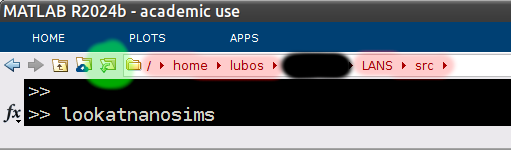
\includegraphics[scale=0.4]{figs1/LANS-startLANS}
\end{center}}

\sbx{Once you are in the correct folder, enter the following command in the Matlab console (see figure above):
\vskip1.5mm\hskip0.5cm
\ttt{lookatnanosims}}

%%% place holder for LANS main gui
\begin{figure}[!t]
\centering
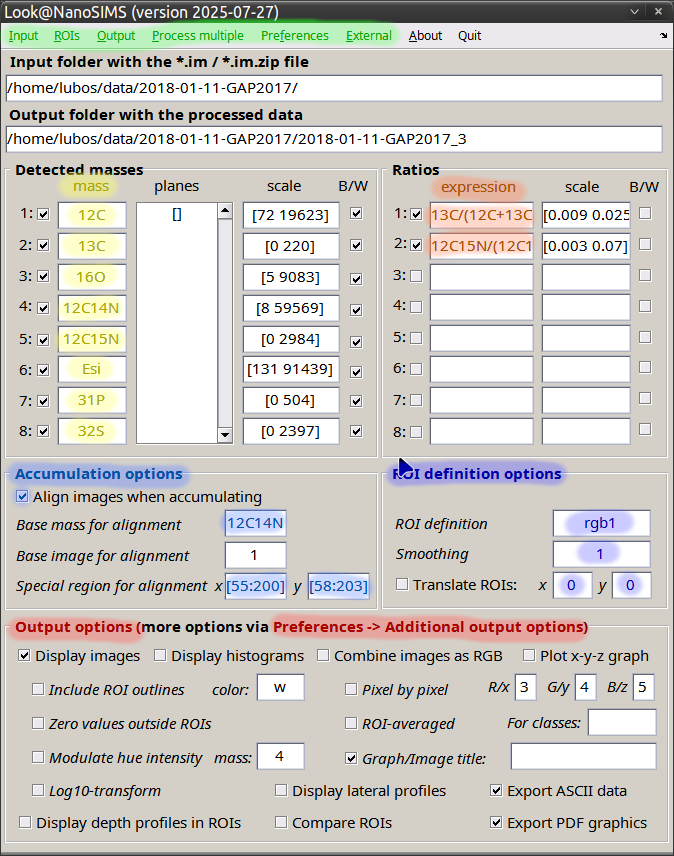
\includegraphics[scale=0.51]{figs1/LANS-maingui}
\caption{\label{fig1:mainLANSgui}%
Main window of the Look@NanoSIMS program. All program functions are executed by selecting an item from the menu (green). Names of the detected \textsf{masses} are filled in automatically during loading of the raw dataset (yellow), \textsf{expressions} for ratios are defined by the user based on the names of the detected masses (orange). Options relevant for drift-correction and accumulation of planes are specificed in the \textsf{Accumulation options} box (light-blue), while those relevant for the definition of ROIs are specified in the \textsf{ROI definition options} box (dark-blue). The most important and frequently changed options defining the {type of analysis} to be performed by LANS, or the {type of output} to be generated, are specified in the \textsf{Output options} box (red). Additional options can be defined through the \textsf{Preferences} menu.}
\end{figure}

\nnb{If everything is set up correctly, the main LANS window will open, as shown in Fig.~\ref{fig1:mainLANSgui}. You can start from there, as described in the following sections of this document.}

\nb{During the data processing session, LANS provides quite a lot of useful information in the Matlab console. Thus, it is a good idea to \textcolor{red}{\emph{always}} keep an eye on the output in the console. You can do this by arranging your desktop such that both the LANS and Matlab console windows are visible at the same time. This is also useful in case you encounter an error while working with LANS. These errors will be shown in the console, too.}

%%

\subsection{Updating LANS}
\setcounter{step}{0}
\goldbox{}
{LANS is updated quite regularly. You can update it easily on your system by entering the following command in the Matlab console:\vskip1.5mm
\hskip0.5cm\ttt{lans\_webupdate}}
\tcbe

\nbx{You need to be in the folder where LANS is installed to run this command. In the process, you will be prompted to make a backup of your older LANS version, which is recommended to do, just in case.}

\nnb{If you are familiar with \ttt{git}, you can update LANS by pulling the latest sources from the LANS github repository \url{https://github.com/lpolerecky/LANS}.}
